\documentclass{beamer}

\setbeamertemplate{button}{\tikz[baseline={(0,-3.5pt)}]
	\node[
	inner xsep=5pt,
	inner ysep=1pt,
	draw=structure!80,
	fill=structure!50,
	rounded corners=4pt]  {\topskip0pt \normalsize\insertbuttontext};}

\usepackage{pgfplots}
\usepackage{cancel}
\usepackage{caption}
\usepackage{dcolumn}
\usepackage{mathtools}
\usepackage{graphicx}
\usepackage{bbm}

\captionsetup{belowskip=-15pt,aboveskip=0pt}

\usepackage{sansmathaccent}

\usenavigationsymbolstemplate{}

\usepackage{array}
\newcolumntype{H}{>{\setbox0=\hbox\bgroup}c<{\egroup}@{}}
\usepackage{makecell}

\makeatletter
\def\thmhead@plain#1#2#3{%
	\thm@notefont{}% same as heading font
	\thmname{#1}\thmnumber{\@ifnotempty{#1}{ }\@upn{#2}}%
	\thmnote{ {\the\thm@notefont#3}}}
\let\thmhead\thmhead@plain
\itshape % body font
\makeatother

%Define normal density function for use in tikzpicture
\pgfmathdeclarefunction{gauss}{2}{%
	\pgfmathparse{3/(#2*sqrt(2*pi))*exp(-((x-#1)^2)/(2*#2^2))}%
}

%This allows adjustable spacing in itemize environment
\newenvironment{wideitemize}{\itemize\addtolength{\itemsep}{10pt}}{\enditemize}

%This allows slide numberering to not includethe title slide
\addtocounter{framenumber}{-1}
\addtobeamertemplate{navigation symbols}{}{%
	\usebeamerfont{footline}%
	\usebeamercolor[fg]{footline}%
	\hspace{1em}%
	%uncomment the below if you want frame numbers inside slide rather than in footline
	%\insertframenumber/\inserttotalframenumber
}

%
\newcommand{\backupbegin}{
	\newcounter{finalframe}
	\setcounter{finalframe}{\value{framenumber}}
}
\newcommand{\backupend}{
	\setcounter{framenumber}{\value{finalframe}}
}

\usetikzlibrary{decorations.pathreplacing,angles,quotes}
\usetikzlibrary{patterns}
\usetikzlibrary{positioning}
\usetikzlibrary{decorations.text}
\usetikzlibrary{decorations.pathmorphing}

%\title{Entangled instrumental variables}
\title{A sample beamer presentation in \LaTeX}

\usetheme{Boadilla}

\subtitle{Using Latex and Beamer}
\author{Pol Dellaiera}
\institute{Institute name here}
\date{\today}

\usepackage{xstring}
\usepackage{catchfile}

\newcommand{\gitfolder}{.git}
\CatchFileDef{\headfull}{\gitfolder/HEAD}{}
\StrGobbleRight{\headfull}{1}[\head]
\StrBehind[2]{\head}{/}[\branch]
\CatchFileDef{\commit}{\gitfolder/refs/heads/\branch}{}
\StrGobbleRight{\commit}{1}[\longcommithash]

\newcommand{\gitrevisionlong}{%
    \longcommithash%
}

\newcommand{\gitrevisionsmall}{%
  \StrLeft{\longcommithash}{7}%
}


\setbeamercovered{}

\begin{document}

\begin{frame}
	\titlepage
	Version {\gitrevisionlong}
\end{frame}

\begin{frame}
    \frametitle{Sample Page 1}
    \[\frac{-b \pm \sqrt{b^2 - c}}{2a}\]
\end{frame}

\begin{frame}
	\frametitle{Sample Page 2}
	\framesubtitle{An Example of Lists}
	\begin{itemize}
		\item 1
		\item 2
		\item 3
	\end{itemize}
\end{frame}

\begin{frame}
    \frametitle{Paragraph Content}
    This is a paragraph.
\end{frame}

\begin{frame}
	\frametitle{Sample frame title}

	In this slide, some important text will be
	\alert{highlighted} because it's important.
	Please, don't abuse it.

	\begin{block}{Remark}
	Sample text
	\end{block}

	\begin{alertblock}{Important theorem}
	Sample text in red box
	\end{alertblock}

	\begin{examples}
	Sample text in green box. The title of the block is ``Examples".
	\end{examples}
\end{frame}

\begin{frame}
	\frametitle{Two-column slide}

	\begin{columns}
		\column{0.5\textwidth}
			This is a text in first column.
			$$E=mc^2$$
			\begin{itemize}
				\item First item
				\item Second item
			\end{itemize}

		\column{0.5\textwidth}
			This text will be in the second column
			and on a second tought this is a nice looking
			layout in some cases.
	\end{columns}
\end{frame}

\begin{frame}{A typical slide}
	Here are some things I want to talk about:\\
	\vspace{.5cm}
	\begin{wideitemize}
		\item Thing 1
		\item Thing 2
		\item Thing 3
	\end{wideitemize}
	\vspace{1cm}
	The above list used \texttt{wideitemize}. Typical \texttt{itemize} spacing:
	\begin{itemize}
		\item Thing 1
		\item Thing 2
		\item Thing 3
	\end{itemize}
\end{frame}


\begin{frame}{Revealing items}
	Here are some things I want to talk about:\\
	\vspace{.5cm}
	\begin{wideitemize}
		\item<1->{Thing 1}
		\item<2->{Thing 2}
		\item<3>{Thing 3}
	\end{wideitemize}
\end{frame}

\begin{frame}{Uncovering items}
	\setbeamercovered{transparent}
	Here are some things I want to talk about:\\
	\vspace{.5cm}
	\begin{wideitemize}
	\item<1>Thing 1
	\item<2->Thing 2
	\item<3>Thing 3
	\end{wideitemize}
\end{frame}

\begin{frame}{You can even plot functions}
	\begin{figure}[h!]
		\begin{tikzpicture}
		\begin{axis}[
		axis x line=bottom,
		axis y line=left,
		xmin=0, xmax=10,
		ymin=0, ymax=5,
		xlabel={$y$},
		ylabel={$\phi(y)$}
		]
		\addplot [fill=gray!80, draw=none, domain=0:10, samples=50] {3*gauss(5,1)} \closedcycle;
		\end{axis}
		\end{tikzpicture}
	\end{figure}
\end{frame}

\begin{frame}{Venn diagram}
	Here's a diagram with the Tikz package: \vspace{.5cm}
	\begin{center}
		\resizebox{4in}{!}{
			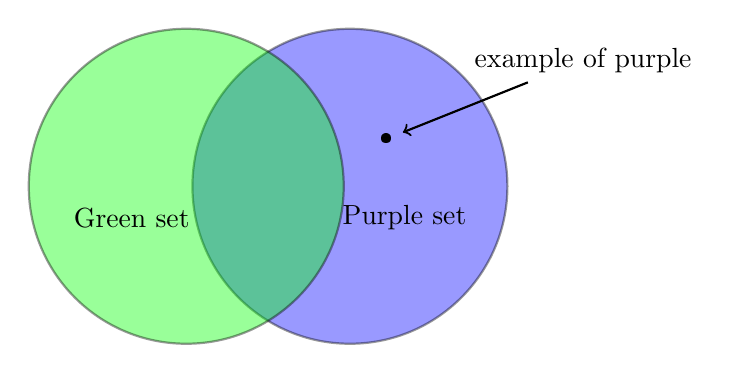
\begin{tikzpicture}[clip=false]
			\fill[blue, draw=black, thick, opacity=.4]  (330:1.2) circle (2);
			\node at ( 330:2)   {Purple set};
			\fill[green, draw=black, thick, opacity=.4] (210:1.2) circle (2);
			\node at ( 210:2)   {Green set};

			\uncover<1->{
				\node (C) at (1.5,0) {\textbullet};
				\node (D) at (4,1) {example of purple};
				\draw[thick,->] (D) -- (C);
			}

			\end{tikzpicture}
		}
	\end{center}
\end{frame}



\end{document}


